\chapter{Die \texorpdfstring{\(SU(5)\)}{5}-Multipletts, Leptoquark-Eichbosonen und Protonenzerfall}

\lectureoverview{Die große Vereinheitlichung wird konkret, wenn die Gruppe des Standardmodells in \(SU(5)\) eingebettet wird. Um zu verstehen, was diese Aussage bedeutet, entwickeln wir zunächst die benötigte Darstellungstheorie: die definierende Darstellung \(N\), ihre konjugierte Darstellung \(\overline N\), Tensorprodukte, symmetrische und antisymmetrische Tensoren sowie die adjungierte Darstellung. Eine Familie des Standardmodells ergibt dann die unerwartet sparsame Kombination \(\overline{\mathbf 5}\oplus\mathbf{10}\). Dieselbe Symmetrie, die diese Anordnung so schön macht, erfordert auch farbgeladene Eichbosonen, die Quarks in Leptonen umwandeln. Ihr Austausch ermöglicht den Protonenzerfall und zwingt die Vereinheitlichungsskala in die Nähe von \(10^{15}\)--\(10^{16}\,\mathrm{GeV}\). Auch die laufenden Eichkopplungen deuten auf eine ähnliche Skala hin; am Ende greifen wir die Supersymmetrie wieder auf, weil sie das numerische Zusammentreffen der Kopplungen deutlich präziser macht.}

\section{Warum beginnen wir mit Gruppendarstellungen?}

Es gibt viele vorgeschlagene große vereinheitlichte Theorien. Statt sie im Überblick zu behandeln, zerlegen wir ein Beispiel und stellen drei Fragen: Was lässt es funktionieren, welche neuen Teilchen erfordert es, und wodurch wird es experimentell gefährdet? Die Gruppe ist \(SU(5)\); ihr wesentliches Strukturmerkmal ist die Einbettung
\begin{equation}
SU(3)_c\times SU(2)_L\times U(1)_Y
\subset SU(5).
\label{eq:l10-sm-embedding}
\end{equation}
Dabei wirkt \(SU(3)_c\) auf die Farbe, \(SU(2)_L\) auf den schwachen Isospin und \(U(1)_Y\) auf die Hyperladung.

Supersymmetrie ist keine Voraussetzung dieser Konstruktion. Weder folgt Supersymmetrie logisch aus der großen Vereinheitlichung, noch folgt die große Vereinheitlichung aus der Supersymmetrie. Ihr Zusammenhang in dieser Vorlesung ist numerischer Art: Bezieht man das Spektrum der Superpartner in die Renormierungsgruppenrechnung ein, nähern sich die drei Eichkopplungen einem gemeinsamen Wert genauer an.

Teilchen, die eine Symmetrie ineinander überführt, bilden eine Darstellung der Symmetriegruppe. Um die vereinheitlichten Teilchenmultipletts zu klassifizieren, benötigen wir daher zunächst einige Grundlagen der Darstellungstheorie.

\subsection{Das bekannte \texorpdfstring{\(SU(2)\)}{SU(2)}-Beispiel}

Die \(SU(2)\), die dem gewöhnlichen Drehimpuls zugrunde liegt, ist eng mit den Drehungen des dreidimensionalen Raums verknüpft. Genauer gesagt ist \(SU(2)\) die zweifache Überlagerungsgruppe von \(SO(3)\). Ihre irreduziblen Darstellungen sind gekennzeichnet durch
\begin{equation}
j=0,\frac12,1,\frac32,\ldots,
\qquad
\dim(j)=2j+1.
\label{eq:l10-su2-spins}
\end{equation}
Ein Skalar ist also ein Singulett, ein Teilchen mit Spin \(\tfrac12\) ein Dublett und ein Teilchen mit Spin eins ein Triplett. Die schwache Gruppe \(SU(2)_L\) ist eine andere physikalische Symmetrie, obwohl ihre abstrakte Gruppentheorie dieselbe ist.

\section{Die definierende Darstellung und ihre konjugierte Darstellung}

Für \(SU(N)\) ist die definierende Darstellung der Raum der komplexen Spalten mit \(N\) Komponenten:
\begin{equation}
\psi=
\begin{pmatrix}
\psi_1\\
\psi_2\\
\vdots\\
\psi_N
\end{pmatrix},
\qquad
\psi'_i=U_i{}^j\psi_j,
\qquad
U\in SU(N).
\label{eq:l10-defining}
\end{equation}
Sie wird als definierende Darstellung oder einfach als \(\mathbf N\) bezeichnet. Die Matrizen \(U\) sind \(N\times N\)-dimensional, und der Vektorraum, auf den sie wirken, hat die Dimension \(N\).

Durch komplexe Konjugation erhält man eine weitere Darstellung mit \(N\) Dimensionen:
\begin{equation}
\psi_i^*\longmapsto U_i{}^{j*}\psi_j^*,
\label{eq:l10-conjugate}
\end{equation}
sie wird mit \(\overline{\mathbf N}\) bezeichnet. Für \(N>2\) sind die definierende Darstellung und die konjugierte Darstellung nicht äquivalent. Man kann die Bezeichnungen für die Teilchendarstellung und die Antiteilchendarstellung vertauschen; hat man sich aber einmal für eine Konvention entschieden, muss man sie beibehalten.

\begin{classroomqa}
\audiencequestion{Hängt das \(N\) in \(SU(N)\) davon ab, ob \(N\) gerade oder ungerade ist, und bezieht es sich auf die Matrizen? \lecturetimestamp{00:07:33}}
\lecturerresponse{Hier gibt es keine Einschränkung auf gerade oder ungerade --. \(N\) gibt die Größe der definierenden Matrizen und zugleich die Dimension ihrer definierenden Darstellung an. Sowohl \(\mathbf N\) als auch \(\overline{\mathbf N}\) haben diese Dimension.}
\end{classroomqa}

Das Antiteilchen eines Antiteilchens ist das ursprüngliche Teilchen. Deshalb ändert die Vertauschung der Bezeichnungen \(\mathbf N\) und \(\overline{\mathbf N}\) die Konvention, nicht aber die Physik.

\section{Tensorprodukte und Irreduzibilität}

Angenommen, ein Objekt kann \(N\) interne Zustände einnehmen und ein anderes Objekt unabhängig davon ebenfalls dieselbe Anzahl. Lassen wir Ort, Impuls, Spin und alle Quantenzahlen außer der Kennzeichnung durch \(SU(N)\) außer Acht, so hat das Paar
\begin{equation}
N\times N=N^2
\label{eq:l10-product-count}
\end{equation}
Zustände. Befindet sich das erste Objekt im Zustand \(\psi_i\) und das zweite im Zustand \(\phi_j\), lässt sich ihr Produkt schreiben als
\begin{equation}
\Psi_{ij}=\psi_i\phi_j,
\qquad
\Psi'_{ij}=U_i{}^kU_j{}^\ell\Psi_{k\ell}.
\label{eq:l10-tensor-transform}
\end{equation}
Dies ist das Tensorprodukt \(\mathbf N\otimes\mathbf N\).

\begin{classroomqa}
\audiencequestion{Warum lautet die Antwort \(N^2\) und nicht \(N^2-1\), und verstößt es gegen das Ausschlussprinzip, wenn beide Teilchen dieselbe interne Kennzeichnung haben dürfen? \lecturetimestamp{00:10:22}}
\lecturerresponse{Die beiden Plätze sind hier unterscheidbar: Ein Objekt befindet sich an einem festen Ort, das andere an einem anderen. Das Pauli-Prinzip schränkt den vollständigen Quantenzustand einschließlich des Orts ein. Es entfernt keine dieser \(N^2\) Kombinationen interner Kennzeichnungen. Die Zahl \(N^2-1\) ergibt sich später aus einer Spurfreiheitsbedingung in einem anderen Produkt.}
\end{classroomqa}

Die Produktdarstellung mit \(N^2\) Dimensionen ist im Allgemeinen reduzibel. Eine Darstellung heißt reduzibel, wenn sie einen echten Unterraum enthält, der von der Gruppe in sich selbst abgebildet wird. Die invarianten Unterräume lassen sich abspalten und als kleinere Darstellungen behandeln; gibt es keinen solchen echten Unterraum, ist die Darstellung irreduzibel.

\subsection{Symmetrische und antisymmetrische Tensoren}

Jeder Tensor mit zwei Indizes lässt sich eindeutig zerlegen in
\begin{align}
\Psi_{ij}
&=\Psi^{(S)}_{ij}+\Psi^{(A)}_{ij},\\
\Psi^{(S)}_{ij}
&=\frac12(\Psi_{ij}+\Psi_{ji}),\\
\Psi^{(A)}_{ij}
&=\frac12(\Psi_{ij}-\Psi_{ji}).
\label{eq:l10-sym-anti}
\end{align}
Die beiden Anteile erfüllen
\begin{equation}
\Psi^{(S)}_{ij}=\Psi^{(S)}_{ji},
\qquad
\Psi^{(A)}_{ij}=-\Psi^{(A)}_{ji}.
\end{equation}
Gleichung~\eqref{eq:l10-tensor-transform} erhält beide Bedingungen; daher führen Gruppentransformationen niemals zu einer Mischung der symmetrischen und antisymmetrischen Sektoren.

\editorialnote{Die Vorlesung überlässt die allgemeine Zählung als Übung. Die Dimensionen der symmetrischen beziehungsweise antisymmetrischen Darstellungen sind \(N(N+1)/2\) und \(N(N-1)/2\); ihre Summe ist \(N^2\).}

\begin{figure}[htbp]
\centering
\includegraphics[width=0.78\textwidth]{lecture_10_figure_02.png}
\lectureframe{00:17:57.500}
\caption{Die fertige Zerlegung von zwei Zuständen mit Spin \(\tfrac12\) an der Tafel: drei symmetrische Zustände und ein antisymmetrischer Zustand.}
\label{fig:l10-spin-decomposition}
\end{figure}

Für das definierende Dublett von \(SU(2)\) gilt:
\begin{equation}
\mathbf2\otimes\mathbf2=\mathbf3_S\oplus\mathbf1_A.
\label{eq:l10-two-two}
\end{equation}
Bezeichnen wir die beiden Basiszustände mit \(u\) und \(d\), so lautet das symmetrische Triplett
\begin{align}
\ket{1,1}&=\ket{uu},\\
\ket{1,0}&=\frac{1}{\sqrt2}\bigl(\ket{ud}+\ket{du}\bigr),\\
\ket{1,-1}&=\ket{dd},
\end{align}
und das antisymmetrische Singulett
\begin{equation}
\ket{0,0}
=\frac{1}{\sqrt2}\bigl(\ket{ud}-\ket{du}\bigr).
\end{equation}
Dies ist die bekannte Addition zweier Drehimpulse mit Spin \(\tfrac12\): Die vier ursprünglichen Zustände ordnen sich zu Spin eins und Spin null.

\section{Ein Teilchen und ein Antiteilchen: die adjungierte Darstellung}

Betrachten wir nun das Produkt der definierenden Darstellung mit ihrer konjugierten Darstellung. Es hat weiterhin \(N^2\) Komponenten, transformiert sich aber wie eine Matrix:
\begin{equation}
M_i{}^j\in\mathbf N\otimes\overline{\mathbf N},
\qquad
M\longmapsto U M U^\dagger.
\label{eq:l10-matrix-transform}
\end{equation}
Anders als bei \(\mathbf N\otimes\mathbf N\) gibt es keine sinnvolle Austauschsymmetrie zwischen einem fundamentalen und einem antifundamentalen Index. Stattdessen bietet sich die Zerlegung an:
\begin{equation}
M
=
\frac{\operatorname{tr}M}{N}\,\mathbf1_N
+
\left(M-\frac{\operatorname{tr}M}{N}\,\mathbf1_N\right).
\label{eq:l10-trace-split}
\end{equation}
Der erste Anteil ist ein Singulett; der spurfreihe Anteil ist die adjungierte Darstellung:
\begin{equation}
\mathbf N\otimes\overline{\mathbf N}
=\mathbf1\oplus\mathbf{Adj},
\qquad
\dim\mathbf{Adj}=N^2-1.
\label{eq:l10-adjoint}
\end{equation}

\begin{figure}[htbp]
\centering
\includegraphics[width=0.67\textwidth]{lecture_10_figure_04.png}
\lectureframe{00:23:47.500}
\caption{Das Ergebnis an der Tafel für \(\mathbf N\otimes\overline{\mathbf N}\): Seine \(N^2-1\) spurfreien Komponenten bilden die adjungierte Darstellung.}
\label{fig:l10-adjoint}
\end{figure}

Für \(SU(3)\) ergibt sich das bekannte Oktett:
\begin{equation}
\mathbf3\otimes\overline{\mathbf3}
=\mathbf8\oplus\mathbf1,
\end{equation}
Die acht Gluonen transformieren in der adjungierten Darstellung. Für \(SU(2)\) hat diese die Dimension drei und transformiert sich wie Spin eins.

\section{Eine Familie des Standardmodells}

Es gibt drei beobachtete Generationen, aber \(SU(5)\) wiederholt dieselbe Konstruktion für jede Generation einzeln. Die Theorie erklärt nicht, warum es drei Kopien gibt. Wir konzentrieren uns daher auf die erste Generation.

Alle Felder werden als linkshändige Weyl-Felder geschrieben. Ein rechtshändiges Fermion wird durch sein linkshändiges ladungskonjugiertes Feld dargestellt:
\begin{equation}
u^c_L,\qquad d^c_L,\qquad e^c_L.
\label{eq:l10-left-handed-bookkeeping}
\end{equation}
Der obere Index \(c\) steht für Ladungskonjugation; beispielsweise ist \(d^c_L\) ein linkshändiges Anti-Down-Feld mit der elektrischen Ladung \(+\tfrac13\).

In der üblichen \(SU(5)\)-Notation passen fünf der fünfzehn linkshändigen Felder in
\begin{equation}
\overline{\mathbf5}
=
\begin{pmatrix}
\nu_{eL}\\
e_L\\
d^c_{rL}\\
d^c_{gL}\\
d^c_{bL}
\end{pmatrix}.
\label{eq:l10-fivebar}
\end{equation}
Die Reihenfolge ist so gewählt, dass auf einen zweidimensionalen schwachen Block ein dreidimensionaler Farbblock folgt. Schwache Transformationen mischen die ersten beiden Einträge, Farbtransformationen die letzten drei, und die nichtdiagonalen \(SU(5)\)-Generatoren verbinden die beiden Blöcke.

\editorialnote{In der Vorlesung wird die Spalte in Gl.~\eqref{eq:l10-fivebar} als \(\mathbf5\) bezeichnet und das antisymmetrische Multiplett später als \(\overline{\mathbf{10}}\). Dies entspricht der global konjugierten Konvention. Wir verwenden die heute übliche Konvention \(\overline{\mathbf5}\oplus\mathbf{10}\); konjugiert man jede Darstellung, erhält man die Bezeichnungen aus der Vorlesung zurück, ohne ihre Physik zu ändern.}

Der vollständige minimale Teilcheninhalt der ersten Generation lautet
\begin{equation}
\begin{gathered}
\underbrace{Q_L=(u_L,d_L)}_{6}
\oplus
\underbrace{L_L=(\nu_{eL},e_L)}_{2},\\
\underbrace{u^c_L}_{3}
\oplus
\underbrace{d^c_L}_{3}
\oplus
\underbrace{e^c_L}_{1},\\
6+2+3+3+1=15.
\end{gathered}
\label{eq:l10-fifteen}
\end{equation}
Das minimale Standardmodell enthält kein unabhängiges \(\nu^c_L\) und liefert daher keine renormierbare Neutrinomasse. Neutrinooszillationen zeigen, dass diese minimale Beschreibung unvollständig ist: In der Natur gibt es kleine, von null verschiedene Neutrinomassen, sodass eine Erweiterung erforderlich ist.

\begin{classroomqa}
\audiencequestion{Wenn eine Fermionmasse einen linkshändigen Zustand in einen rechtshändigen überführt, wird das Teilchen dann zugleich zu seinem Antiteilchen? \lecturetimestamp{00:34:00}}
\lecturerresponse{Nein. Eine Elektronenmasse verbindet ein linkshändiges Elektron mit einem rechtshändigen Elektron derselben elektrischen Ladung. In der Notation, in der alle Felder linkshändig sind, wird das zweite Feld durch \(e^c_L\) dargestellt; das Vierkomponententeilchen bleibt jedoch ein Elektron. Nur ein neutrales Feld kann eine Majorana-Masse haben, die Teilchen und Antiteilchen miteinander identifiziert.}
\end{classroomqa}

\section{Eichbosonen im Fünfer-Multiplett}

Zu jedem Generator einer Eichsymmetrie gehört ein Eichfeld. In ~\eqref{eq:l10-fivebar} lassen sich die bekannten Übergänge bereits erkennen:
\begin{itemize}
\item Die schwachen Eichfelder wirken zwischen \(\nu_{eL}\) und \(e_L\);
\item die Gluonen wirken zwischen den drei Farben von \(d^c_L\);
\item neutrale Generatoren wirken diagonal;
\item neue nichtdiagonale Generatoren wandeln einen Leptoneintrag in einen farbigen Eintrag um oder umgekehrt.
\end{itemize}

Man kann sich das Gluon so vorstellen, dass es Farquantenzahlen eines Quark--Antiquark-Paars trägt. Die Vorlesung verwendet die übliche Weltlinien-Merkhilfe: Verfolgt man ein auslaufendes Antiquark durch den Emissionsvertex rückwärts, sieht es wie ein vorwärts laufendes Quark aus. Das emittierte Feld trägt somit die Quantenzahlen eines Quark--Antiquark-Paars. In der Sprache der Darstellungen ist dies genau der spurfreie Anteil von \(\mathbf3\otimes\overline{\mathbf3}\).

Für \(SU(5)\) gilt
\begin{equation}
\dim\mathbf{Adj}_{SU(5)}=5^2-1=24.
\end{equation}
Die Zerlegung dieser Eichfelder bezüglich der Untergruppe des Standardmodells lautet
\begin{equation}
\mathbf{24}
=
(\mathbf8,\mathbf1)_0
\oplus(\mathbf1,\mathbf3)_0
\oplus(\mathbf1,\mathbf1)_0
\oplus(\mathbf3,\mathbf2)_{-5/6}
\oplus(\overline{\mathbf3},\mathbf2)_{5/6},
\label{eq:l10-adjoint-sm}
\end{equation}
wobei das geordnete Paar \(SU(3)_c\times SU(2)_L\) bezeichnet und der Index die Hyperladung angibt.

\editorialnote{Gleichung~\eqref{eq:l10-adjoint-sm} macht die in der Vorlesung gezeichnete Blockstruktur explizit. Die ersten drei Terme enthalten die bekannten Farb- und elektroschwachen Eichfelder. Die letzten beiden Terme entsprechen den zwölf reellen Freiheitsgraden, die man üblicherweise \(X\)- und \(Y\)-Bosonen nennt.}

\begin{figure}[htbp]
\centering
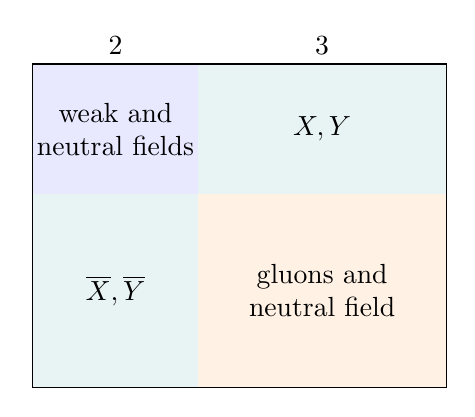
\begin{tikzpicture}[x=1.05cm,y=0.82cm]
  \draw[thick] (0,0) rectangle (5,5);
  \draw[thick] (2,0) -- (2,5);
  \draw[thick] (0,3) -- (5,3);
  \fill[blue!9] (0,3) rectangle (2,5);
  \fill[orange!10] (2,0) rectangle (5,3);
  \fill[teal!9] (2,3) rectangle (5,5);
  \fill[teal!9] (0,0) rectangle (2,3);
  \node[align=center] at (1,4) {weak and\\neutral fields};
  \node[align=center] at (3.5,1.5) {gluons and\\neutral field};
  \node[align=center] at (3.5,4) {\(X,Y\)};
  \node[align=center] at (1,1.5) {\(\overline X,\overline Y\)};
  \node[above] at (1,5) {\(2\)};
  \node[above] at (3.5,5) {\(3\)};
\end{tikzpicture}
\caption{Die \(2\oplus3\)-Blockstruktur des \(SU(5)\)-Eichfelds. Die nichtdiagonalen Blöcke verbinden Leptonen und farbige Felder.}
\label{fig:l10-gauge-blocks}
\end{figure}

Mit \(Q=T_3+Y\) hat das farbige schwache Dublett in ~\eqref{eq:l10-adjoint-sm} die Ladungen \(-\tfrac13\) und \(-\tfrac43\); das konjugierte Dublett hat die Ladungen \(+\tfrac13\) und \(+\tfrac43\). Die Vorlesung nennt diese Teilchen \(X\) und \(Y\), legt aber ausdrücklich nicht fest, welche Bezeichnung zu welcher Ladung gehört. Der Übergang und die Ladung sind der invariante Inhalt.

\begin{classroomqa}
\audiencequestion{Gibt es von jedem neuen \(X\)- oder \(Y\)-Eichboson drei Varianten? \lecturetimestamp{00:41:28}}
\lecturerresponse{Ja. Ein Übergang verbindet einen farbigen Quarkeintrag mit einem farblosen Leptoneintrag; das ausgetauschte Boson muss daher die fehlende Farbe tragen. Die \(X/Y\)-Felder bilden Farbtripletts und können Gluonen emittieren oder absorbieren.}
\end{classroomqa}

Farbige Teilchen werden nicht als isolierte asymptotische Zustände beobachtet. Die neuen Eichbosonen müssen in farbneutrale Kombinationen zerfallen oder hadronisieren, so wie Quarks.

\section{Warum das Multiplett Anti-Down-Quarks enthält}

Die Generatoren von \(SU(N)\) sind spurfreie hermitesche Matrizen. Um den Zusammenhang mit der Bezeichnung „speziell“ zu erkennen, schreiben wir ein infinitesimales Gruppenelement als
\begin{equation}
U(\epsilon)=e^{i\epsilon T}.
\end{equation}
Aus der Unitarität folgt \(T^\dagger=T\), während
\begin{equation}
1=\det U=e^{i\epsilon\operatorname{tr}T}
\end{equation}
für beliebiges \(\epsilon\) ergibt:
\begin{equation}
\operatorname{tr}T=0.
\label{eq:l10-traceless-generator}
\end{equation}

Die elektrische Ladung ist eine Linearkombination von Generatoren. Auf die Materiespalte in ~\eqref{eq:l10-fivebar} wirkt sie als
\begin{equation}
Q_{\overline5}
=
\operatorname{diag}
\left(0,-1,\frac13,\frac13,\frac13\right),
\qquad
\operatorname{tr}Q_{\overline5}=0.
\label{eq:l10-charge-fivebar}
\end{equation}
Damit gilt
\begin{equation}
0-1+3\left(\frac13\right)=0.
\end{equation}
Ersetzte man die Anti-Down-Felder durch Down-Felder, ergäbe sich stattdessen
\begin{equation}
0-1+3\left(-\frac13\right)=-2,
\end{equation}
Dies kann nicht die Spur eines \(SU(5)\)-Generators sein. Die auf den ersten Blick ungewöhnliche Zuordnung der Anti-Down-Felder ist somit durch die Gruppenstruktur erzwungen.

\section{Die übrigen zehn Fermionen}

Die übrigen zehn Felder stammen aus einem antisymmetrischen Tensor mit zwei Indizes. In der üblichen Konvention ist dies der antisymmetrische Anteil von
\begin{equation}
\mathbf5\otimes\mathbf5
=\mathbf{15}_S\oplus\mathbf{10}_A.
\label{eq:l10-five-five}
\end{equation}
Die Vorlesung konstruiert ihn, indem sie vorübergehend die konjugierten Quantenzahlen notiert:
\begin{equation}
\chi=
\begin{pmatrix}
\nu^c\\
e^c\\
d_r\\
d_g\\
d_b
\end{pmatrix}.
\label{eq:l10-aux-five}
\end{equation}
Dies ist eine Buchführungshilfe für das Tensorprodukt von Darstellungen und keine Behauptung, dass ein zweites physikalisches Fünfer-Multiplett zusammengesetzter Teilchen existiert.

Sei
\begin{equation}
\Psi^{ij}=-\Psi^{ji},
\qquad
i,j=1,\ldots,5.
\label{eq:l10-antisym-ten}
\end{equation}
Alle Diagonaleinträge verschwinden, und das untere Dreieck ist durch das obere festgelegt. Daher gilt
\begin{equation}
\dim\mathbf{10}
=\binom52
=\frac{5\cdot4}{2}
=10.
\label{eq:l10-ten-count}
\end{equation}

Die elektrische Ladung eines Eintrags ist die Summe der Ladungen von Zeile und Spalte in ~\eqref{eq:l10-aux-five}. Daraus folgen unmittelbar \(e^c\) im Schwach--Schwach-Feld, Down- und Up-Quarks in den Schwach--Farb-Blöcken sowie Anti-Up-Felder im Farb--Farb-Block.

\begin{classroomqa}
\audiencequestion{Müsste der resultierende Eintrag ein \(X\)-Boson sein, wenn man die Bezeichnungen Positron und Down-Quark kombiniert? \lecturetimestamp{00:53:08}}
\lecturerresponse{Nein. In diesem Schritt konstruieren wir die Fermiondarstellung, nicht die adjungierte Darstellung der Eichbosonen. Die Ladungen addieren sich zu \(1-\tfrac13=\tfrac23\); der Eintrag hat also die Quantenzahlen eines Up-Quarks.}
\end{classroomqa}

Eine konsistente Wahl der Farbvorzeichen lautet
\begin{equation}
\Psi^{ij}=
\begin{pmatrix}
0 & e^c & d_r & d_g & d_b\\
-e^c & 0 & u_r & u_g & u_b\\
-d_r & -u_r & 0 & u_b^c & -u_g^c\\
-d_g & -u_g & -u_b^c & 0 & u_r^c\\
-d_b & -u_b & u_g^c & -u_r^c & 0
\end{pmatrix}.
\label{eq:l10-ten-matrix}
\end{equation}
Änderungen der Feldphasen verändern manche dargestellten Vorzeichen, nicht aber die Darstellung oder den Teilcheninhalt.

\begin{figure}[htbp]
\centering
\includegraphics[width=0.83\textwidth]{lecture_10_figure_05.png}
\lectureframe{00:59:17.500}
\caption{Die vollständig ausgefüllte antisymmetrische Materiematrix in der \(2\oplus3\)-Zerlegung, nachdem die Einträge und Farbkennzeichnungen im Unterricht überprüft wurden.}
\label{fig:l10-ten-board}
\end{figure}

\begin{classroomqa}
\audiencequestion{Muss die zehn-dimensionale Darstellung als Matrix geschrieben werden, oder lässt sie sich auch als Spalte darstellen? \lecturetimestamp{00:56:24}}
\lecturerresponse{Beides ist möglich. Man kann die zehn unabhängigen Komponenten als Spalte auflisten; die antisymmetrische \(5\times5\)-Matrix zeigt jedoch, wie \(SU(5)\) auf ihre beiden Indizes wirkt, und ist deshalb wesentlich aussagekräftiger.}
\end{classroomqa}

\begin{classroomqa}
\audiencequestion{Müsste der mit \(u\) gekennzeichnete Eintrag im Farb--Farb-Block eigentlich ein Anti-Up-Feld sein? \lecturetimestamp{00:57:51}}
\lecturerresponse{Ja. Die Beschriftung an der Tafel wird zu \(u^c\) korrigiert, einem linkshändigen Anti-Up-Feld. Die Ladungen zweier Down-Basiszustände ergeben \(-\tfrac23\), also die elektrische Ladung eines Anti-Up-Quarks.}
\end{classroomqa}

\begin{classroomqa}
\audiencequestion{Bei mehreren Matrixeinträgen fehlen die Farben. Bleiben sie trotzdem erhalten? \lecturetimestamp{00:58:05}}
\lecturerresponse{Ja. Die drei Farbplätze stehen für Rot, Grün und Blau. Die Kennzeichnungen wurden nur weggelassen, um die Darstellung übersichtlicher zu halten.}
\end{classroomqa}

Ein antisymmetrisches Paar fundamentaler Farbzustände transformiert sich wie eine Antifarbe:
\begin{equation}
\wedge^2\mathbf3\simeq\overline{\mathbf3},
\qquad
(rg,rb,gb)\sim(\overline b,-\overline g,\overline r).
\label{eq:l10-anticolor}
\end{equation}
Deshalb bilden die drei unabhängigen Einträge im Farb--Farb-Block genau das Anti-Up-Farbtriplett.

Eine Generation ist nun wie folgt angeordnet:
\begin{equation}
\overline{\mathbf5}\oplus\mathbf{10}.
\label{eq:l10-family}
\end{equation}
Bemerkenswert ist, dass \(u_L\) und \(u^c_L\) zum selben irreduziblen Multiplett gehören, während \(d_L\) und \(d^c_L\) beziehungsweise \(e_L\) und \(e^c_L\) in verschiedenen Multipletts liegen.

\begin{classroomqa}
\audiencequestion{Wenn Eichtransformationen nur innerhalb jeder Darstellung wirken, wie kann eine Masse dann Felder verbinden, die im Fünfer-Antimultiplett und im Zehner liegen? \lecturetimestamp{01:00:40}}
\lecturerresponse{Eichbosonen überführen nicht eine irreduzible Materiedarstellung in die andere. Higgs-Felder und Yukawa-Kopplungen können verschiedene Darstellungen miteinander verbinden und dabei eine insgesamt \(SU(5)\)-invariante Wechselwirkung bilden. Nimmt das Higgs-Feld einen Erwartungswert an, erzeugen diese Wechselwirkungen Massen.}
\end{classroomqa}

\section{Eichbosonen wirken als Verschiebungen}

Nachdem das Multiplett zusammengestellt ist, lässt sich die Wirkung eines Eichbosons als Verschiebung zwischen seinen Einträgen lesen. Ein neutrales Boson kann eine Kennzeichnung unverändert lassen, ein schwaches Boson wechselt zwischen schwachen Plätzen, ein Gluon zwischen Farbplätzen und ein \(X/Y\)-Boson zwischen schwachen und Farbplätzen. Geladene Eichbosonen haben Antiteilchen, daher gibt es zu jeder Verschiebung auch den umgekehrten Prozess.

Auf den antisymmetrischen Tensor wirkt eine infinitesimale Transformation auf beide Indizes:
\begin{equation}
\delta\Psi^{ij}
=
i\epsilon
\left(
T^i{}_k\Psi^{kj}
+
T^j{}_k\Psi^{ik}
\right).
\label{eq:l10-two-index-action}
\end{equation}
Im Matrixbild verschiebt der erste Term vertikal und der zweite horizontal. Die Teilchenbezeichnungen, mit denen der Tensor aufgebaut wird, dienen nur als Merkstütze; ~\eqref{eq:l10-two-index-action} ist die exakte gruppentheoretische Aussage.

Schwache Verschiebungen überführen \(d\) in \(u\) – dies ist der Prozess auf Quarkebene, der dem Betazerfall des Neutrons zugrunde liegt. Farbverschiebungen ändern Rot, Grün und Blau, ohne den Flavour zu verändern. Nichtdiagonale Verschiebungen bewirken etwas Neues:
\begin{equation}
\begin{aligned}
d^c&\longleftrightarrow e,
& d^c&\longleftrightarrow\nu,\\
d&\longleftrightarrow u^c,
& u&\longleftrightarrow e^c,
\end{aligned}
\label{eq:l10-leptoquark-shifts}
\end{equation}
wobei das passende \(X/Y\)-Feld die Differenz in Ladung und Farbe trägt.

\begin{classroomqa}\audiencequestion{Was bedeuten Verschiebungen zwischen dem vierten und fünften Eintrag, und was ist mit einer Verschiebung vom ersten zum vierten? \lecturetimestamp{01:10:36}}
\lecturerresponse{Die Verschiebung vom vierten--fünften Eintrag wandelt eine Farbe in eine andere um und entspricht einem Gluonübergang. Eine Verschiebung vom ersten--vierten Eintrag führt zwischen dem schwachen und dem Farbbereich hindurch und entspricht einem der neuen \(X/Y\)-Übergänge.}
\end{classroomqa}

\begin{classroomqa}
\audiencequestion{Kann ein Eintrag in der unteren Hälfte der antisymmetrischen Matrix explizit ausgefüllt werden? \lecturetimestamp{01:11:23}}
\lecturerresponse{Ja. Jeder Eintrag im unteren Dreieck ist das Negative des transponierten Eintrags im oberen Dreieck. Füllt man einen Eintrag aus, wird die Regel sichtbar; alle übrigen auszufüllen ergibt keine neuen Zustände.}
\end{classroomqa}

\section{Die gefährliche Folge: Protonenzerfall}

Ein \(X/Y\)-Boson kann an einem Vertex ein Quark mit einem Lepton und an einem anderen zwei quarkartige Felder koppeln. Bei Impulsen, die viel kleiner als seine Masse sind, ergibt das Integrieren über das schwere Boson eine Wechselwirkung der Dimension sechs mit der schematischen Form
\begin{equation}
\mathcal L_{\mathrm{eff}}
\sim
\frac{g_5^2}{M_X^2}\,(qq)(q\ell)
+\text{h.c.}
\label{eq:l10-effective-proton}
\end{equation}
Sie verletzt die Baryonenzahl und die Leptonenzahl einzeln, erhält aber die Kombinationen, die durch die vereinheitlichte Eichwechselwirkung vorgegeben sind.

An der Tafel wird verfolgt, wie ein Down-Quark und ein Up-Quark durch den Austausch des schweren Bosons umgewandelt werden. Das Down-Quark wird zum Positron, das Up-Quark zum Anti-Up-Quark, während ein zweites Up-Quark als Zuschauer unverändert bleibt:
\begin{equation}
uud
\longrightarrow
e^++u\overline u.
\label{eq:l10-quark-decay}
\end{equation}
Der Anfangszustand ist ein Proton. Das Paar \(u\overline u\) kann zu einem neutralen Pion hadronisieren; damit ergibt sich
\begin{equation}
p\longrightarrow e^++\pi^0.
\label{eq:l10-proton-pion}
\end{equation}

\begin{figure}[htbp]
\centering
\includegraphics[width=0.82\textwidth]{lecture_10_figure_06.png}
\lectureframe{01:16:02.500}
\caption{Die fertige Konstruktion des Austauschs eines schweren Bosons im Proton an der Tafel, mit dem Zuschauer-Up-Quark und dem Positronkanal.}
\label{fig:l10-proton-board}
\end{figure}

Die Vorlesung erwähnt außerdem \(p\to e^++\gamma\), bei dem das Quark--Antiquark-Paar elektromagnetisch annihiliert. Dieser Kanal ist im Vergleich zur direkten Hadronisierung zusätzlich elektromagnetisch unterdrückt.

Diese Möglichkeit ist keine optionale Ergänzung des Modells. Sobald eine einfache Gruppe Generatoren enthält, die Quarks und Leptonen verbinden, sind Prozesse zu erwarten, die die Baryonenzahl verletzen. Würden sie auf gewöhnlichen schwachen oder elektromagnetischen Zeitskalen ablaufen, blieben weder Atomkerne noch Wasserstoff oder makroskopische Materie erhalten.

\section{Warum ist das Proton so langlebig?}

\begin{classroomqa}
\audiencequestion{Ist die Kopplung, die ein \(X\)-Boson erzeugt, dieselbe vereinheitlichte Kopplung wie für den Rest der Gruppe? \lecturetimestamp{01:18:34}}
\lecturerresponse{Auf der Vereinheitlichungsskala: ja. Eine einfache Eichtheorie mit \(SU(5)\) hat eine einzige Eichkopplung \(g_5\). Die niederenergetischen Kopplungen der starken und der schwachen Wechselwirkung sowie der Hyperladung unterscheiden sich, weil sie sich nach dem Brechen der vereinheitlichten Symmetrie unterschiedlich entwickeln.}
\end{classroomqa}

Die Kopplung kann nicht beliebig klein gewählt werden, ohne die vereinheitlichte Struktur aufzugeben. Die verfügbare Unterdrückung stammt vom schweren Propagator:
\begin{equation}
\mathcal A
\sim
\frac{g_5^2}{M_X^2}.
\label{eq:l10-amplitude}
\end{equation}
Das Quadrieren der Amplitude liefert den Faktor \(g_5^4/M_X^4\). Eine Dimensionsanalyse zusammen mit dem Protonenmatrixelement ergibt die Abschätzung der Zerfallsrate:
\begin{equation}
\Gamma_p
\sim
C_{\mathrm{had}}\,
\frac{\alpha_5^2\,m_p^5}{M_X^4},
\qquad
\alpha_5=\frac{g_5^2}{4\pi},
\label{eq:l10-rate}
\end{equation}
wobei \(C_{\mathrm{had}}\) Gruppenfaktoren, Renormierungseffekte und das nichtperturbative hadronische Matrixelement enthält.

\editorialnote{Die Vorlesung hebt die wesentliche Abhängigkeit von \(g^4/M_X^4\) hervor und weist darauf hin, dass Faktoren mit Protonmassen ausgelassen sind. Gleichung~\eqref{eq:l10-rate} stellt die erforderliche Massendimension wieder her, ohne eine präzise Berechnung der Lebensdauer zu beanspruchen.}

\begin{classroomqa}
\audiencequestion{Reicht der kleine Faktor \(g^4\), in der groben Abschätzung an der Tafel etwa von der Größenordnung \(10^{-8}\), bereits aus, um die Lebensdauer groß genug zu machen? \lecturetimestamp{01:25:13}}
\lecturerresponse{Nein. Er trägt dazu bei, doch zwischen einer mikroskopischen Zeitskala der starken Wechselwirkung und der Schranke für die Protonlebensdauer liegen sehr viel mehr Größenordnungen. Die vierte Potenz der schweren Masse muss die entscheidende Unterdrückung liefern.}
\end{classroomqa}

Wären alle Massen von der Größenordnung der Protonmasse, wäre die natürliche Zeiteinheit ungefähr die Lichtlaufzeit durch ein Proton:
\begin{equation}
t_p\sim\frac{1\ \mathrm{fm}}{c}\sim10^{-23}\ \mathrm{s}.
\label{eq:l10-proton-time}
\end{equation}
Schon die bloße Existenz primordialer Protonen zeigt, dass ihre Lebensdauer das Alter des Universums übersteigt; Laborsuchen gehen jedoch sehr viel weiter. Die Vorlesung vergleicht die mikroskopische Abschätzung mit der damals angegebenen experimentellen Grenze
\begin{equation}
\tau_p\gtrsim10^{33}\ \mathrm{yr}.
\label{eq:l10-lifetime-bound}
\end{equation}

Man muss nicht ein einzelnes Proton so lange beobachten. Betrüge die Lebensdauer \(10^{15}\) Jahre, würde eine Probe mit \(10^{15}\) Protonen ungefähr ein Ereignis pro Jahr ergeben. Allgemeiner ist für \(N_p\) beobachtete Protonen während einer Zeit \(T\) die erwartete Zahl der Zerfälle
\begin{equation}
\langle n\rangle\simeq\frac{N_pT}{\tau_p}.
\label{eq:l10-event-count}
\end{equation}
Ein Detektor mit ungefähr \(10^{33}\) Protonen ist ein großer Tank, kein astronomisches Objekt: Die Protonen selbst haben eine Masse von etwa \(10^6\) Kilogramm. Durch die Beobachtung einer solchen Probe lässt sich eine enorme individuelle Lebensdauer in eine messbare Ereignisrate oder eine strengere untere Schranke umwandeln.

Kombiniert man ~\eqref{eq:l10-rate} mit der Lebensdauerbedingung, ergibt sich für die Masse des Leptoquark-Eichbosons ungefähr
\begin{equation}
M_X\sim10^{15}\text{--}10^{16}\ \mathrm{GeV},
\label{eq:l10-mx}
\end{equation}
wobei die Vorlesung \(10^{16}\,\mathrm{GeV}\) als einprägsame, sichere Skala verwendet. Diese liegt mehrere Größenordnungen unterhalb der Planck-Skala und ist daher nicht automatisch mit der Quantenfeldtheorie unvereinbar.

\section{Brechung von \texorpdfstring{\(SU(5)\)}{SU(5)} und die Vereinheitlichungsskala}

Die \(X/Y\)-Felder gehören zusammen mit den Eichfeldern des Standardmodells zu einem adjungierten \(SU(5)\)-Multiplett. Bei einer exakt ungebrochenen Eichsymmetrie könnten einige seiner Mitglieder nicht Massen nahe \(10^{16}\,\mathrm{GeV}\) haben, während Photon und Gluonen masselos bleiben. Die Symmetrie muss also spontan gebrochen werden.

\begin{classroomqa}
\audiencequestion{Wären alle Eichbosonen von \(SU(5)\) masselos, wenn diese Symmetrie ungebrochen wäre? \lecturetimestamp{01:29:37}}
\lecturerresponse{Ja, in der hier betrachteten Eichtheorie. Die Eichinvarianz verbietet eine explizite gemeinsame Masse. Ein Higgs-Mechanismus kann den Eichbosonen gebrochener Generatoren Massen verleihen, während die Eichfelder der ungebrochenen Untergruppe masselos bleiben.}
\end{classroomqa}

Der elektroschwache Higgs-Mechanismus veranschaulicht dieses Muster bereits: Er unterscheidet das Photon von \(W^\pm\) und \(Z\). Die große Vereinheitlichung erfordert einen eigenen Ordnungsparameter auf hoher Skala, der den schwachen \(2\)-Block vom Farb\(3\)-Block unterscheidet und die nichtdiagonalen \(X/Y\)-Felder extrem schwer macht.

Verglichen mit \(10^{16}\,\mathrm{GeV}\) ist selbst eine Masse des schwachen Bosons von \(100\,\mathrm{GeV}\) vernachlässigbar. Weit oberhalb der Schwelle der schweren Teilchen können alle Eichbosonmassen vernachlässigt werden; dann ist die volle \(SU(5)\)-Symmetrie eine gute Näherung. Das bedeutet Vereinheitlichungsskala: Die niederenergetische Welt weist nicht sichtbar \(SU(5)\) auf, aber Prozesse bei hinreichend hohen Energien werden unempfindlich gegenüber den durch Symmetriebrechung verursachten Massendifferenzen.

\section{Laufende Kopplungen}

Eichkopplungen hängen logarithmisch von der Energieskala ab. Definiert man
\begin{equation}
\alpha_i(\mu)=\frac{g_i^2(\mu)}{4\pi},
\end{equation}
so hat die Entwicklung in einer Schleife die Form
\begin{equation}
\alpha_i^{-1}(\mu)
=
\alpha_i^{-1}(\mu_0)
-\frac{b_i}{2\pi}
\ln\!\left(\frac{\mu}{\mu_0}\right).
\label{eq:l10-running}
\end{equation}
Die Koeffizienten \(b_i\) hängen von der Eichgruppe und von jedem Teilchen ab, das leicht genug ist, um in den betreffenden Quantenschleifen aufzutreten.

\editorialnote{Damit sich die Hyperladung mit den nichtabelschen Kopplungen innerhalb von \(SU(5)\) vergleichen lässt, muss \(g_1\) die übliche Normierung großer vereinheitlichter Theorien erhalten. Daher stammen die in der Vorlesung erwähnten numerischen gruppentheoretischen Faktoren.}

Bei Laborenergien unterscheiden sich die Kehrwerte der drei Kopplungen. In der qualitativen Reihenfolge der Vorlesung ist \(1/\alpha_1\) am größten, weil die Hyperladung am schwächsten ist; danach folgt \(1/\alpha_2\), und \(1/\alpha_3\) ist am kleinsten, weil die starke Wechselwirkung am stärksten ist. Die Kurven bei unzugänglichen Energien werden nicht direkt gemessen. Sie werden aus den beobachteten Niederenergiewerten, dem Teilchenspektrum und den Schleifendiagrammen berechnet, die die Betafunktionen bestimmen. Beim Teilcheninhalt des Standardmodells ergeben sich nahezu gerade Linien, wenn man sie gegen \(\log\mu\) aufträgt.

\begin{figure}[htbp]
\centering
\includegraphics[width=0.74\textwidth]{lecture_10_figure_07.png}
\lectureframe{01:36:32.500}
\caption{Tafelgrafik, auf der sich die inversen Eichkopplungen bei etwa \(10^{16}\,\mathrm{GeV}\) einander annähern. Der eingekreiste Bereich markiert, dass sie sich nicht exakt treffen.}
\label{fig:l10-running-board}
\end{figure}

Unterhalb der Vereinheitlichungsschwelle ist die Symmetrie gebrochen, das leichte Spektrum bildet keine vollständigen entarteten \(SU(5)\)-Multipletts, und die drei Betafunktionskoeffizienten unterscheiden sich. Daher ändern sich die Kopplungen mit unterschiedlicher Rate. Auf der hohen Energieskala stellt sich die Frage, ob sie einen gemeinsamen Wert erreichen:
\begin{equation}
\alpha_1(M_{\mathrm{GUT}})
\stackrel{?}{=}
\alpha_2(M_{\mathrm{GUT}})
\stackrel{?}{=}
\alpha_3(M_{\mathrm{GUT}}).
\label{eq:l10-unification-condition}
\end{equation}

Allein mit dem nichtsupersymmetrischen Spektrum des Standardmodells nähern sich die Linien bei etwa \(10^{15}\)--\(10^{16}\,\mathrm{GeV}\) einander an, verfehlen den gemeinsamen Wert jedoch deutlich; die Vorlesung beschreibt die Übereinstimmung als ungefähr fünfzehn Prozent. Die wichtige Koinzidenz besteht darin, dass dies zugleich die von der Protonstabilität geforderte Skala ist.

\section{Eine abschließende Frage zum Neutron}

\begin{classroomqa}
\audiencequestion{Wenn man im Protonzerfallsdiagramm das zuschauende Up-Quark durch ein Down-Quark ersetzte, würde dies einen Neutronzerfall beschreiben, und wäre das \(X\)-Boson dabei von Bedeutung? \lecturetimestamp{01:36:40}}
\lecturerresponse{Damit wäre ein großvereinheitlichter Neutronzerfallskanal wie \(n\to e^++\pi^-\) definiert, aber das ist nicht der vertraute Zerfall eines freien Neutrons. Der gewöhnliche Betazerfall des Neutrons lautet \(n\to p+e^-+\overline\nu_e\) und läuft über die schwache Wechselwirkung ab. Wäre die Massenordnung von Proton und--Neutron umgekehrt, wäre auch die Betastabilität umgekehrt, während der viel langsamere großvereinheitlichte Zerfallskanal weiterhin bestehen könnte.}
\end{classroomqa}

Diese Unterscheidung trennt die Kinematik von der neuen Wechselwirkung. Welches Nukleon einem Betazerfall unterliegt, hängt von der Massendifferenz zwischen Proton und--Neutron ab; die Baryonenzahlverletzung durch den Austausch von \(X/Y\) ist ein davon unabhängiger, extrem stark unterdrückter Mechanismus.

\section{Supersymmetrie und der größere Zusammenhang}

Ein supersymmetrisches Partnerspektrum verändert die Betafunktionskoeffizienten in Gl.~\eqref{eq:l10-running}. Der Darstellung in der Vorlesung zufolge treffen sich die drei extrapolierten Kopplungen dann mit einer Genauigkeit von etwa einem Prozent. Das beweist weder Supersymmetrie noch große Vereinheitlichung, ist aber der empirische Grund dafür, dass beide Ideen oft gemeinsam diskutiert werden.

Die Materiemultipletts lassen sich noch weiter vereinheitlichen. Es gilt:
\begin{equation}
SO(10)\supset SU(5),
\end{equation}
Eine Spinordarstellung zerfällt in
\begin{equation}
\mathbf{16}
\longrightarrow
\mathbf{10}\oplus\overline{\mathbf5}\oplus\mathbf1.
\label{eq:l10-so10}
\end{equation}
Der Singulettzustand lässt sich auf natürliche Weise mit einem linkshändigen Antineutrino oder gleichbedeutend mit dem ladungskonjugierten Zustand eines rechtshändigen Neutrinos identifizieren. Damit passen alle sechzehn Felder einer erweiterten Familie in ein einziges irreduzibles \(SO(10)\)-Multiplett.

Protonzerfallsexperimente prüfen die Idee weiterhin, indem sie die untere Schranke für die Lebensdauer anheben, wenn kein Ereignis beobachtet wird. Supersymmetrische großvereinheitlichte Modelle sagen keine universelle Protonlebensdauer voraus: zusätzliche schwere Felder und von den Superpartnern abhängige Operatoren können den dominanten Zerfallskanal und die Zerfallsrate in einem weiten Bereich verändern.

\editorialnote{In der supersymmetrischen großen Vereinheitlichung kann der Austausch farbgeladener Higgs-Triplets zusätzlich zum hier besprochenen Eichbosonoperator der Dimension sechs baryonenzahlverletzende Operatoren der Dimension fünf erzeugen. Ihre Koeffizienten hängen stark vom schweren Spektrum, der Flavourstruktur und den Superpartner-Massen ab. Das erklärt die Warnung in der Vorlesung, dass sich aus Supersymmetrie allein keine einzelne Lebensdauer ergibt.}

Die bleibende Lehre ist ein Spannungsverhältnis, kein abschließendes Urteil. Die Gruppentheorie vereint Quarks und Leptonen mit bemerkenswerter Eleganz, die laufenden Kopplungen deuten auf eine gemeinsame hohe Skala hin, und die Supersymmetrie schärft diesen numerischen Hinweis. Dieselbe Konstruktion sagt auch die gefährliche Umwandlung von Quarks in Leptonen voraus. Jede erfolgreiche Version muss daher die Eleganz bewahren und zugleich das Proton für nahezu unvorstellbar lange Zeit stabil halten. Im Sinne des Schlussworts der Vorlesung: Mögen all unsere Protonen stabil bleiben.
